% Build with xetex.
\documentclass[aspectratio=43,handout,bigger]{beamer}

%% -------------------------------------------------------------------------- %%

\usepackage{xunicode}
\usepackage{xltxtra}
\usepackage{graphicx}

\usepackage{color}

\usepackage{setspace}
\usepackage{ragged2e}

\usepackage[normalem]{ulem}

\usepackage{minted}

\usepackage{tikz}
\usetikzlibrary{shapes,arrows,chains,calc,fit,matrix}

%% -------------------------------------------------------------------------- %%

\usepackage{polyglossia}
\setmainlanguage{russian}
\setotherlanguage{english}

% NB: To get MS fonts for OS X:
%
% 1) Install MS Open XML Converter.
% 2) Install OpenXML_all_fonts.pkg from inside of Converter's mpkg.
%
% http://www.labnol.org/software/tutorials/\
% free-download-calibri-font-on-mac/3684/

\setmainfont{Calibri}
\setsansfont{Calibri}
\setmonofont{Consolas}

%% -------------------------------------------------------------------------- %%

\mode<presentation>{
  \usetheme{default}
}

\useinnertheme{circles}

\setbeamertemplate{navigation symbols}{}
\setbeamertemplate{section in toc}[sections numbered]

\definecolor{chart11}{RGB}{0, 0, 0}
\setbeamercolor{title}{fg=chart11}
\setbeamercolor{author}{fg=chart11}
\setbeamercolor{frametitle}{fg=chart11}
\setbeamercolor{itemize item}{fg=chart11}
\setbeamercolor{itemize subitem}{fg=chart11}
\setbeamercolor{itemize subsubitem}{fg=chart11}
\setbeamercolor{section in toc}{fg=chart11}

\setbeamersize{text margin left=0.5cm,text margin right=0.5cm}

%% -------------------------------------------------------------------------- %%

\defbeamertemplate{footline}{left page number}
{%
  \hfill
  \usebeamercolor[fg]{page number in head/foot}%
  \usebeamerfont{page number in head/foot}%
  \insertpagenumber\,/\,\insertpresentationendpage%
  \hspace*{1em}
  \vskip1em%
}
\setbeamertemplate{footline}[left page number]

%% ========================================================================== %%

\title{
\includegraphics[height=.15\textheight]{logo}}
\author{Quick functional UI sketches\\with Lua templates and mermaid.js}
\institute{Alexander Gladysh\\@agladysh}
\date{Lua in Moscow / Devconf 2017}

%% ========================================================================== %%

\begin{document}

% Using [plain] to avoid frame number on the title page.
\begin{frame}[plain]
 \titlepage
\end{frame}

%% ========================================================================== %%

\begin{frame}{Talk plan}

\tableofcontents

\end{frame}

%% ========================================================================== %%

\section*{}

\begin{frame}{About me}

\begin{itemize}
\item Programmer background
\item Mainly doing management work now
\item In löve with Lua since 2005
\end{itemize}

\end{frame}

%% ========================================================================== %%
\section{The Case}
%% ========================================================================== %%

\begin{frame}{The Case}
  \begin{itemize}
    \item A huge professional enterprise application
    \item being converted from 20-year-old windows app
    \item to a modern SPA web-app.
  \end{itemize}
\end{frame}

%% -------------------------------------------------------------------------- %%

\begin{frame}{The product is huge}
  Sufficient expertise can only be found on a team level:

  \begin{itemize}
    \item Technology experts don't have product-level vision
    \item PO and PM don't draw professionally
          (and lack deep insight on the tech)
    \item Designer does not have the professional-level technology expertise
  \end{itemize}
\end{frame}

%% -------------------------------------------------------------------------- %%

\begin{frame}{The UI design and development process}
  For each "screen" in the application:

  \begin{itemize}
    \item Concept
    \item Functional sketches and (sometimes) interactive studies
    \item Design sketches
    \item Layout implementation
    \item Business logic implementation
  \end{itemize}
\end{frame}

%% -------------------------------------------------------------------------- %%

\begin{frame}{A functional sketch}
  What is on the screen, how does it WORK?

  \centering{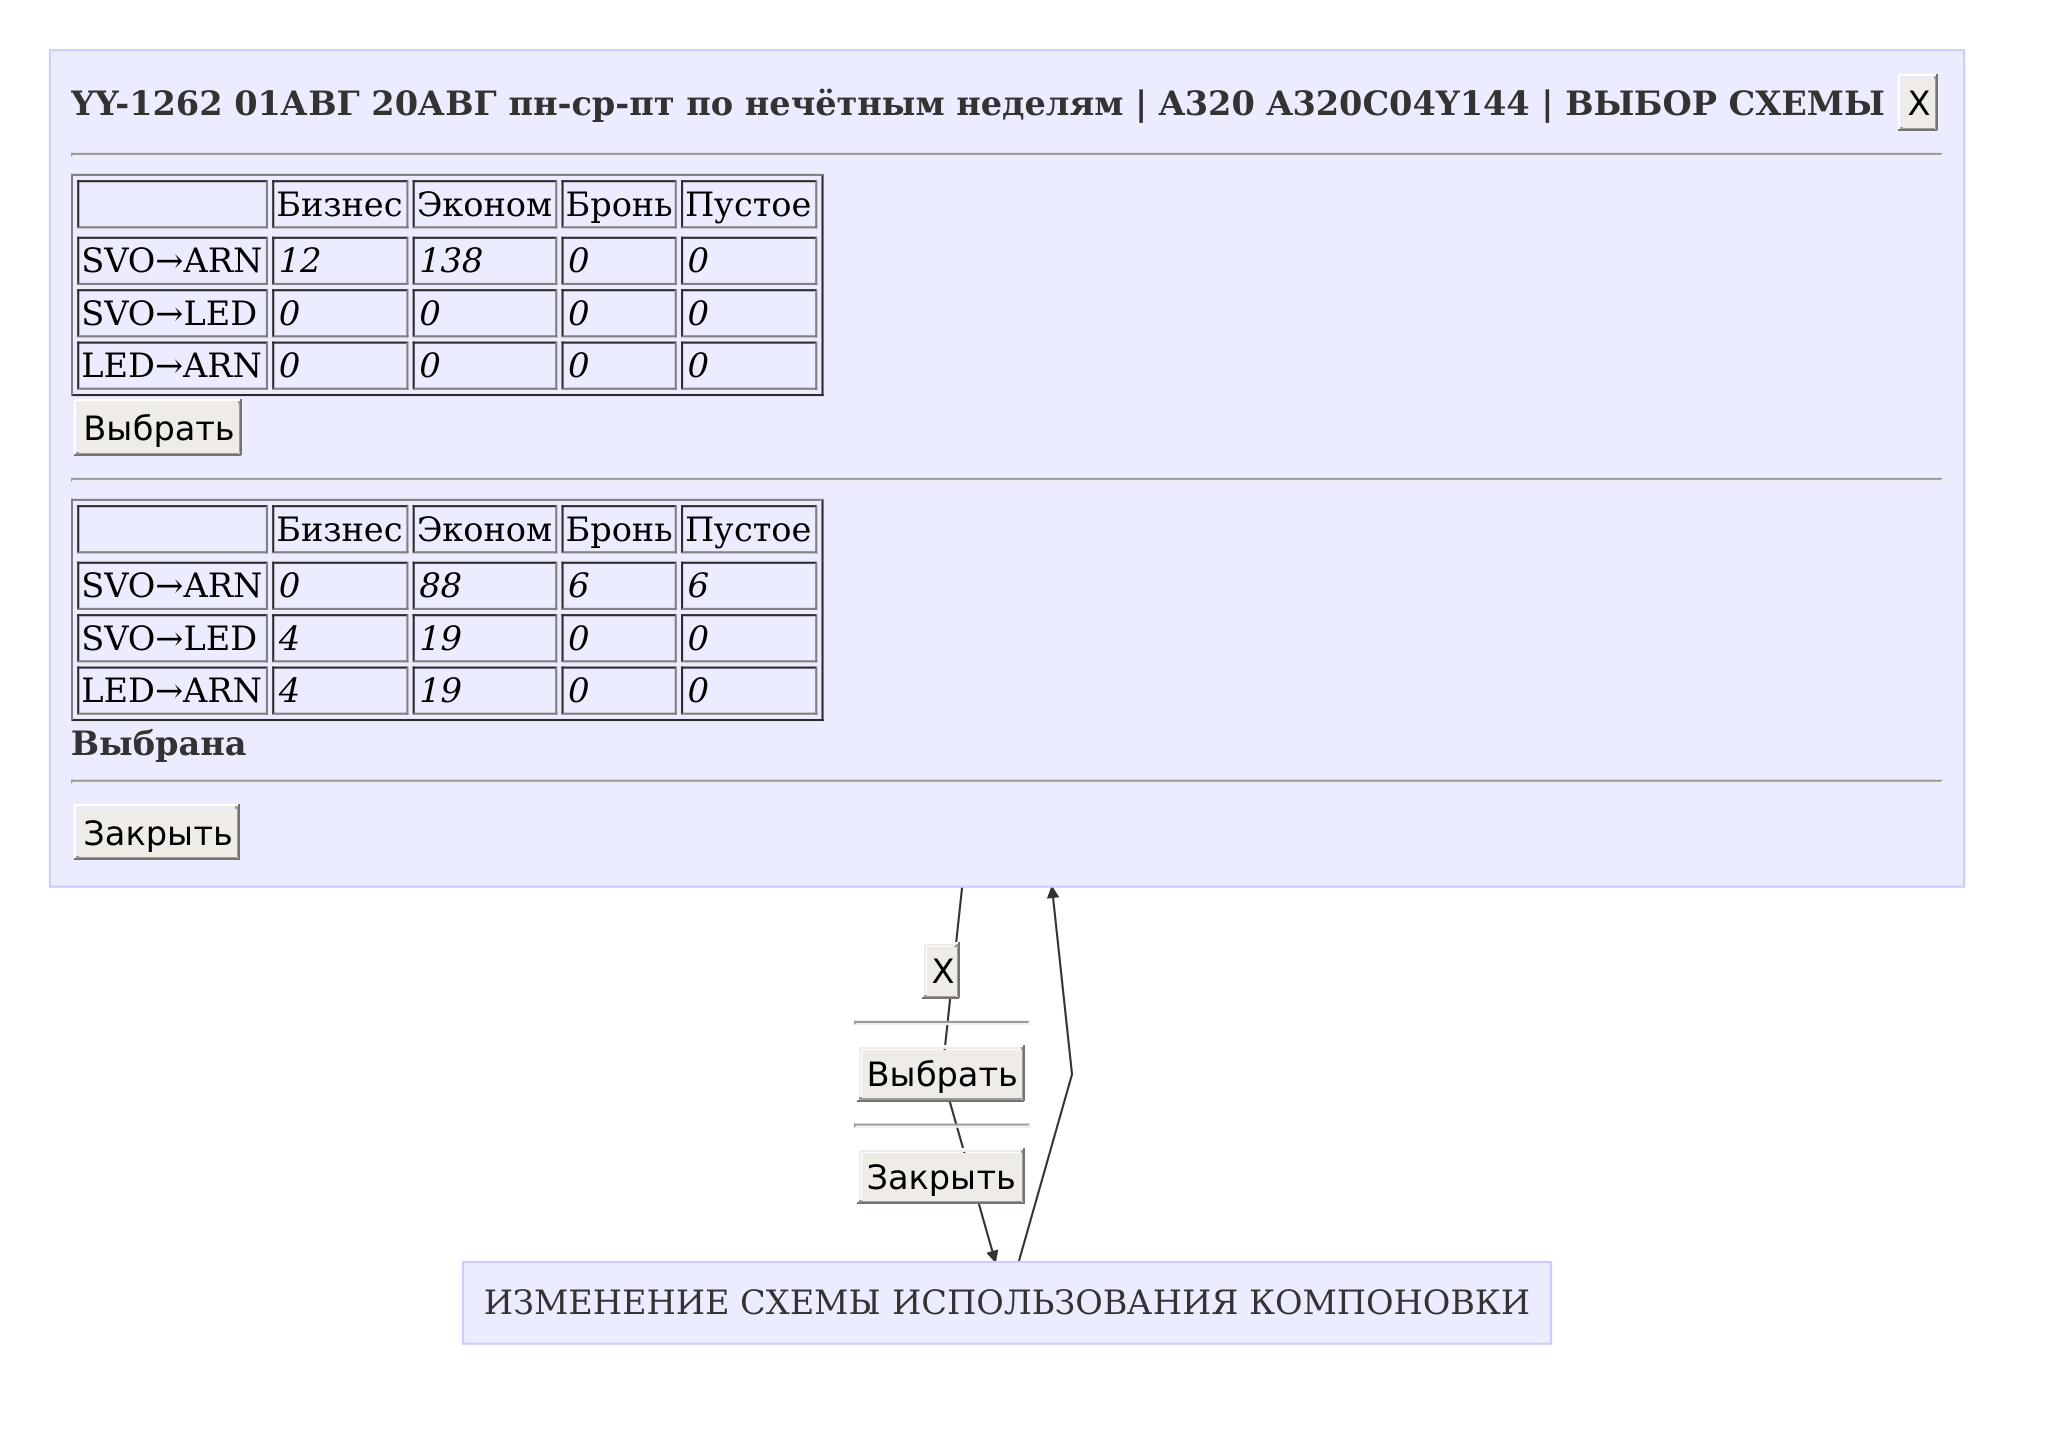
\includegraphics[height=.75\textheight]{seatmap}}
\end{frame}

%% -------------------------------------------------------------------------- %%

\begin{frame}{A design sketch}
  How does it LOOK?

  \centering{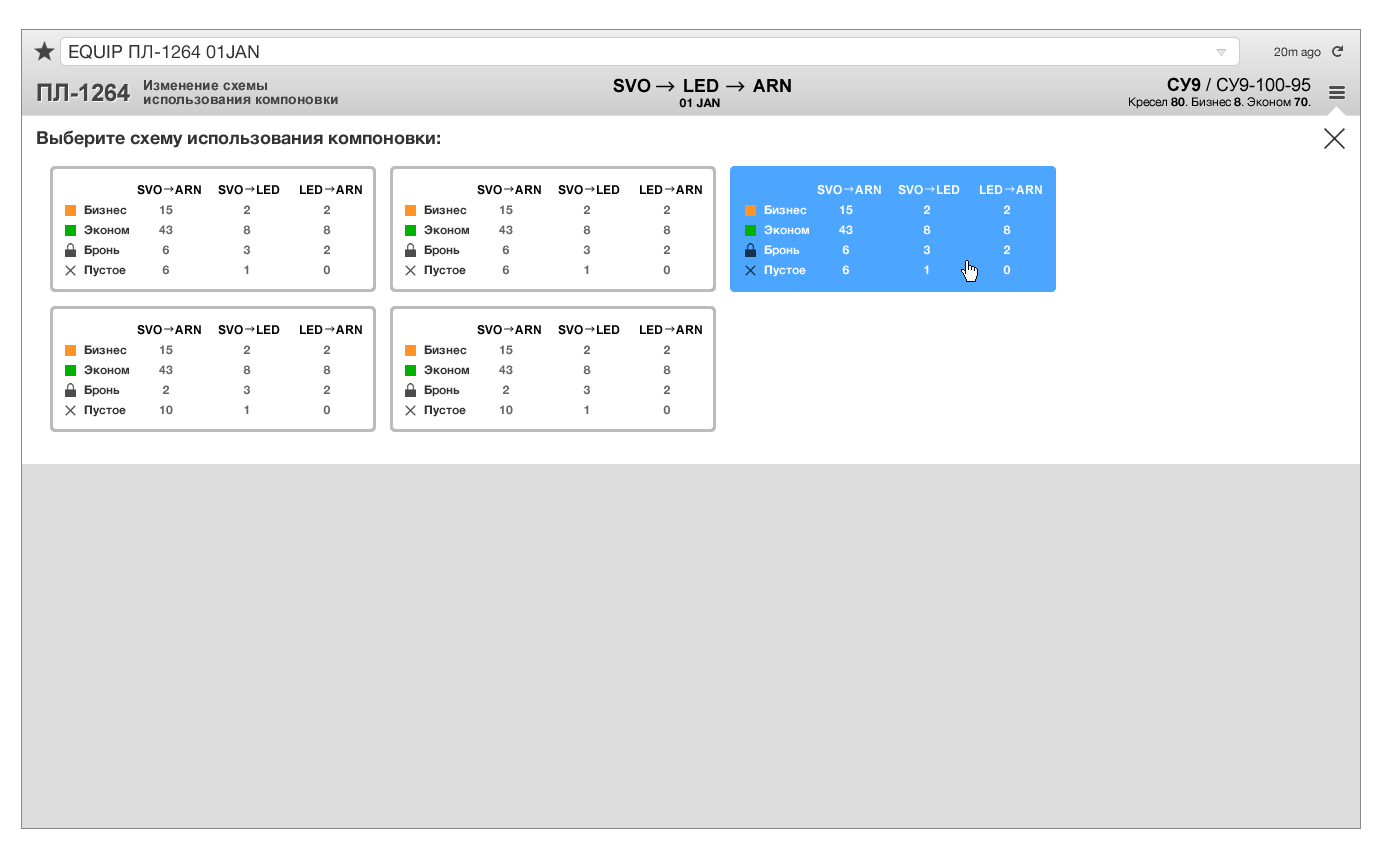
\includegraphics[height=.75\textheight]{EQUIP-1_2}}
\end{frame}

%% -------------------------------------------------------------------------- %%

\begin{frame}{Goals}
  \begin{itemize}
    \item I need a diagram of the flow between app screens
    \item I need functional sketches of the screens themselves
    \item Basically it doesn't matter how I make them as long
          as they are easy to make and change and there are some
          facilities for reuse.
  \end{itemize}
\end{frame}

%% ========================================================================== %%
\section{Approaches to design}
%% ========================================================================== %%

\begin{frame}{What tools to use?}
  \begin{itemize}
    \item Photoshop (Krita, Gimp...)
    \item InkScape
    \item Google Documents
    \item Visio
    \item Balsamiq
    \item Sketch
    \item ...
  \end{itemize}
  \vskip 1em
  I'm a programmer, I'm better with structured text than with images.
  \vskip 1em
  I work fastest with the keyboard, not having to touch the mouse.
\end{frame}

%% ========================================================================== %%
\section{Enter the Mermaid}
%% ========================================================================== %%

\begin{frame}{Enter the Mermaid}
  http://bit.ly/mermaid-editor

  \centering{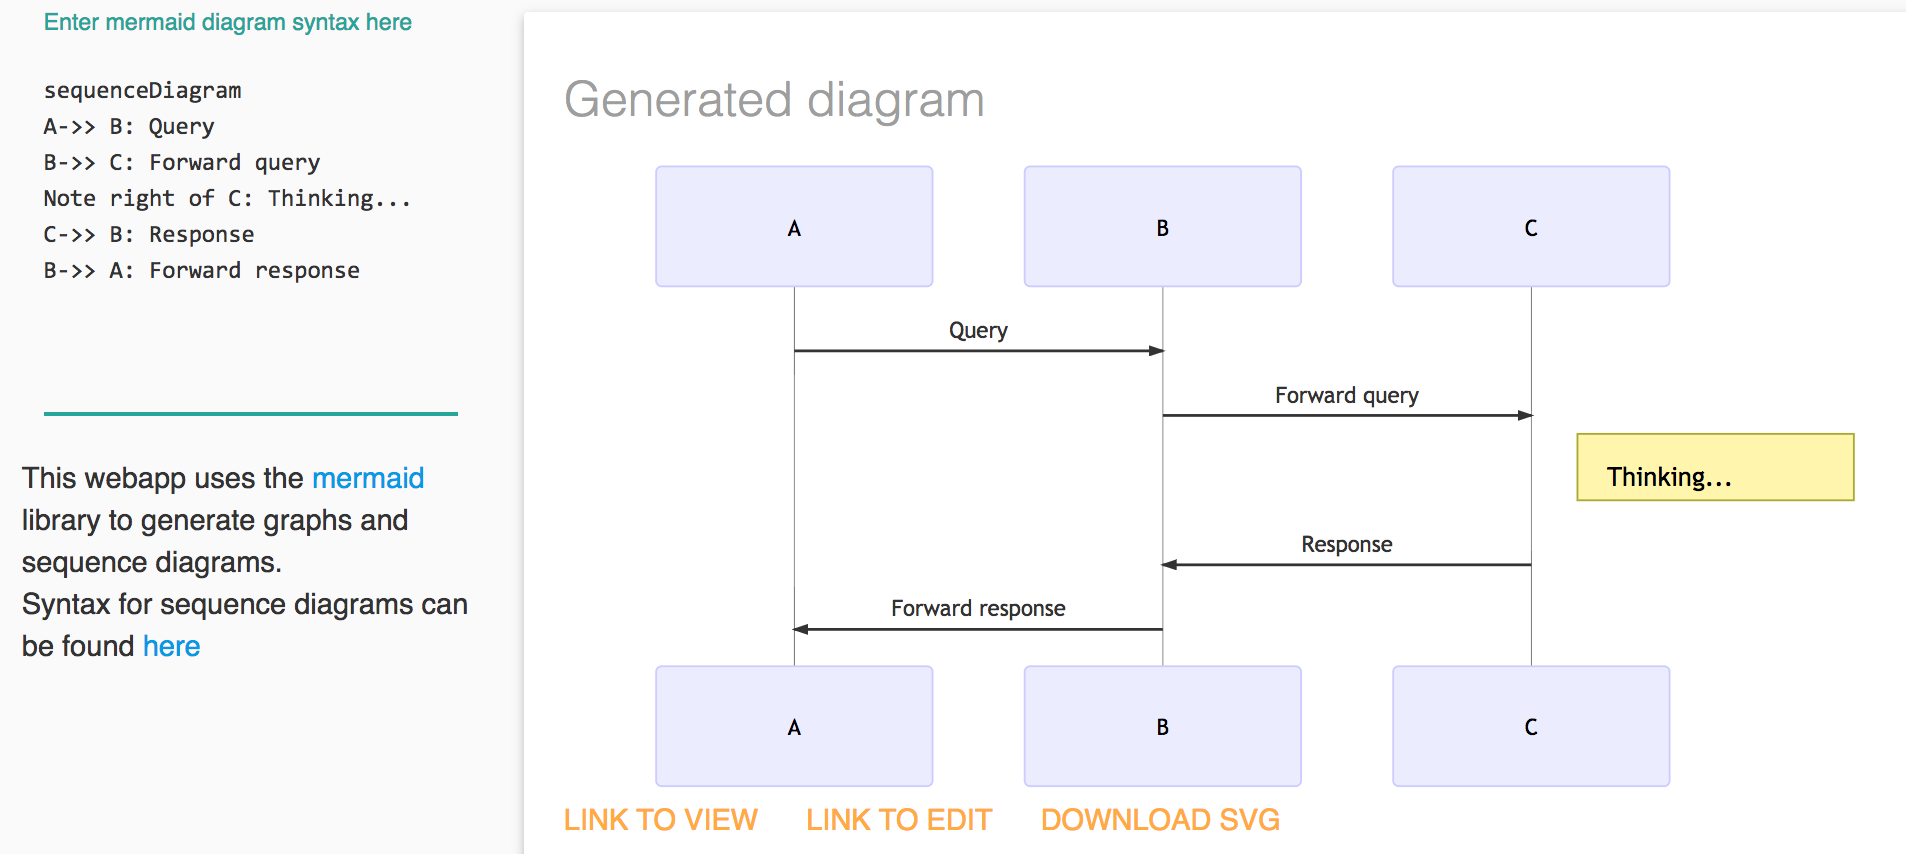
\includegraphics[width=.95\textwidth]{liveeditor}}
\end{frame}

%% -------------------------------------------------------------------------- %%

\begin{frame}[fragile]{Screen Flow Diagram}
  \begin{columns}
    \begin{column}{.5\textwidth}
\begin{minted}{text}
graph TD

list[List of Flights]
new[New Flight Form]

list-->|Create|new
\end{minted}
\end{column}
\begin{column}{.5\textwidth}
\centering{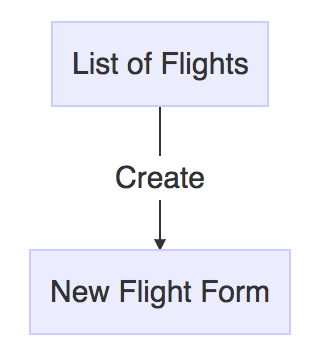
\includegraphics[width=\textwidth]{flights-1}}
\end{column}
\end{columns}
\end{frame}

%% -------------------------------------------------------------------------- %%

\begin{frame}[fragile]{Screen Flow Diagram (II)}
  \begin{columns}
    \begin{column}{.5\textwidth}
\begin{minted}{html}
graph TD

list[List of Flights]
new[New Flight Form]

list-->|"
<button>Create</button>
"|new
\end{minted}
\end{column}
\begin{column}{.5\textwidth}
\centering{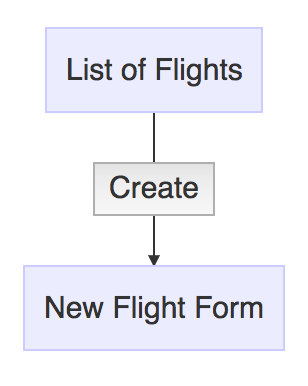
\includegraphics[width=\textwidth]{flights-2}}
\end{column}
\end{columns}
\end{frame}

%% -------------------------------------------------------------------------- %%

\begin{frame}[fragile]{Screen Prototypes}
  \begin{columns}
    \begin{column}{.5\textwidth}
\begin{minted}{text}
graph TD

list["<b>List of Flights</b>
    <hr>
    <i>(No flights)</i><hr>
    <button>Create</button>"]

new["New Flight Form"]
list-->|"
<button>Create</button>
"|new
\end{minted}
  \end{column}
  \begin{column}{.5\textwidth}
    \centering{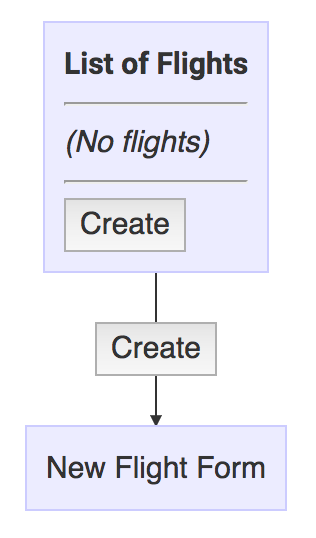
\includegraphics[height=.9\textheight]{flights-3}}
  \end{column}
  \end{columns}
\end{frame}

%% -------------------------------------------------------------------------- %%

\begin{frame}[fragile]{Screen Prototypes (II)}
  \begin{columns}
    \begin{column}{.6\textwidth}
\begin{minted}{text}
graph TD
list["List of Flights"]
new["<b>New Flight</b><hr>
<input value='SU' size='2'>-
<input value='2618' size='4'><br>
<input value='MOW' size='5'> to
<input value='BRU' size='5'><br>
<input value='20:50' size='5'> to
<input value='22:30' size='5'>
<hr><button>Create</button>
<u>Cancel</u>"]
new-->|"
<button>Create</button>"|list
new-->|"<u>Cancel</u>"|list
\end{minted}
    \end{column}
    \begin{column}{.3\textwidth}
      \centering{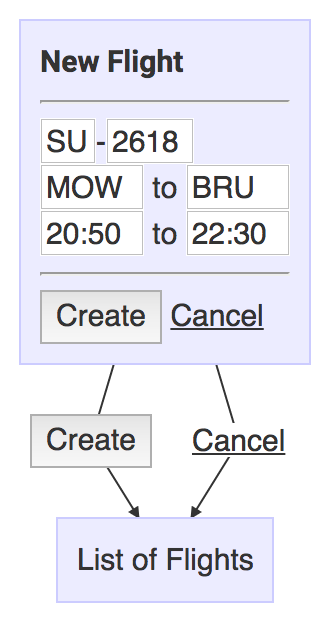
\includegraphics[width=\textwidth]{flights-4}}
    \end{column}
  \end{columns}
\end{frame}

%% -------------------------------------------------------------------------- %%

\begin{frame}{Basic Documentation Structure}
  \centering{
    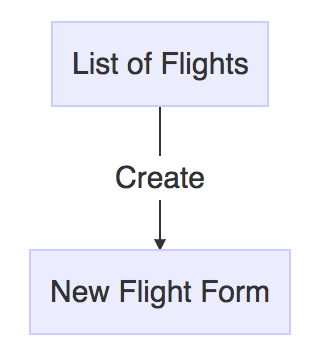
\includegraphics[width=.3\textwidth]{flights-1}
    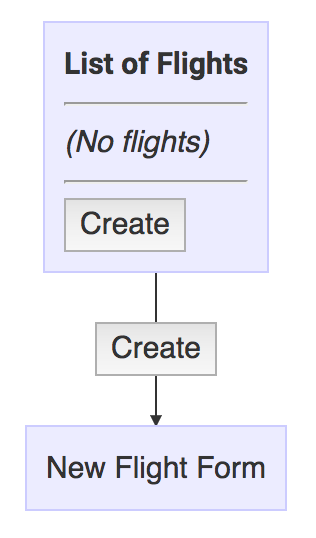
\includegraphics[width=.3\textwidth]{flights-3}
    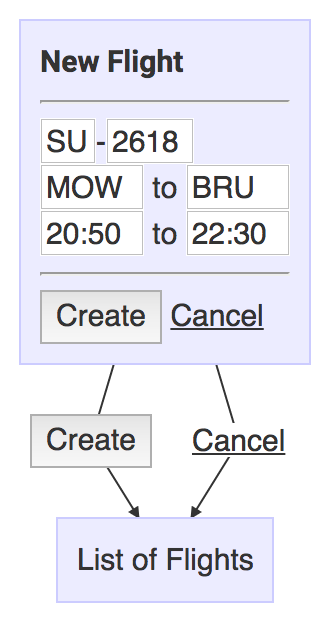
\includegraphics[width=.3\textwidth]{flights-4}
  }
\end{frame}

%% -------------------------------------------------------------------------- %%

\begin{frame}[fragile]{It is hard to do HTML without templates: list}
\begin{minted}{text}
<b>${title List of Flights}</b><hr>

<i>(No flights)</i><hr>

${link new <button>Create</button>}
\end{minted}
\end{frame}

%% -------------------------------------------------------------------------- %%

\begin{frame}[fragile]{It is hard to do HTML without templates: new}
\begin{minted}{text}
<b>${title New Flight}</b><hr>

<input value='SU' size='2'>-
<input value='2618' size='4'><br>

<input value='MOW' size='4'> to
<input value='BRU' size='4'><br>

<input value='20:50' size='5'> to
<input value='10:30' size='5'><hr>

${link list <button>Create</button>}
${link list <button>Cancel</button>}
\end{minted}
\end{frame}

%% ========================================================================== %%
\section{Lugram Templates}
%% ========================================================================== %%

\begin{frame}[fragile]{Basic helpers}
\begin{minted}{text}
${title New Flight}
\end{minted}

  \${title <text:*>}

  \vskip 1em

\begin{minted}{text}
${link list <button>Create</button>}
\end{minted}

  \${link <screen:word> <body:*>}
\end{frame}

%% -------------------------------------------------------------------------- %%

\begin{frame}[fragile]{Basic helpers: pass-through definitions}
\begin{minted}{text}
${define title {{'*', 'text'}} [[${text}]]}

${title New Flight} --> New Flight
\end{minted}

\vskip 1em

\begin{minted}{text}
${define link
  {{'word', 'target'}, {'*', 'body'}}
  [[${body}]]}

${link list <button>Create</button>}
--> <button>Create</button>
\end{minted}

\vskip 1em

\${define <symbol:word> <arguments:table> <code:*>}
\end{frame}

%% -------------------------------------------------------------------------- %%

\begin{frame}[fragile]{define}
\begin{minted}{lua}
define = function(context, str)
  local symbol, str = eat.word(str)
  local args, str = eat.table(str)
  local code, str = eat['*'](str)
  args, code = lua_value(args), lua_value(code)
  if type(code) == 'string' then code =
    function(ctx) return ctx:replace(code) end
  end
  context._ROOT[symbol] = function(parent, str)
    local ctx = { }
    for i = 1, #args do
      ctx[args[i][1]], str = eat[args[i][2]](str)
    end
    return code(parent:push(ctx))
  end
end
\end{minted}
\end{frame}

%% -------------------------------------------------------------------------- %%

\begin{frame}[fragile]{helpers: definitions using Lua}
\begin{minted}{text}
${define title {{'*', 'text'}} function(context)
  local text = context:replace(context.text)
  context._ROOT._SCREENS[text] = text
  return text
end}
\end{minted}

\begin{minted}{text}
${define link {{'word', 'target'}, {'*', 'body'}}
function(context)
  local target = context:replace(context.text)
  context._ROOT._LINKS[target] = context._MODULE
  context:include(target) -- Ignoring result
  return context:replace(context.body)
end}
\end{minted}
\end{frame}

%% -------------------------------------------------------------------------- %%

\begin{frame}[fragile]{include}
\begin{minted}{lua}
include = function(context, template)
  return context:push(
    { _MODULE = template }
  ):replace(
    assert(io.open(filename)):read("*a")
  )
end
\end{minted}
\end{frame}

%% -------------------------------------------------------------------------- %%

\begin{frame}{Diagram styles}
  Depending on how you define \${title} and \${link},
  you get several kinds of diagram from the same set of templates:

  \begin{itemize}
    \item Outline diagram (titles and arrows only, "screen flow")
    \item Closeup diagram (screen content and flow from this screen to others)
    \item Printable diagram (screen content only)
  \end{itemize}
\end{frame}

%% -------------------------------------------------------------------------- %%

\begin{frame}[fragile]{More Useful helpers}
\begin{minted}{text}
${define # {{'*', 'comment'}} [[]]}
${define --[HR]------...--------- {} [[<hr>]]}

${define expr {{'*', 'code'}} function(context)
  return assert(loadstring('return '
    .. context:replace(context.code)))()
end}
\end{minted}
\end{frame}

%% -------------------------------------------------------------------------- %%

\begin{frame}[fragile]{with helper}
\begin{minted}{text}
${define with {{'table', 'more_context'},
  {'*', 'body'}} function(context)
  return context:replace(
    context:push(context.more_context),
    context.body)
end}

${define form {} [[
  ${when editable
    <input value='MOW'> to <input value='BRU'>}
  ${unless editable MOW to BRU}
]]}

${with {editable = true} ${form}}
\end{minted}
\end{frame}

%% -------------------------------------------------------------------------- %%

\begin{frame}[fragile]{with helper (II)}
\begin{minted}{html}
${define histogram {{'word', 'a'},
  {'word', 'b'}, {'word', 'c'}} [[
${with { w = '${expr ${a} + ${b} + {c}}' }
  <div style='width:${w}px' class='red'>
    <div style='width:${a}px'
      class='green'>${a}</div>
    <div style='width:${b}px'
      class='blue'>${b}</div>
  </div>
}]]}

${histogram 1 2 3}
\end{minted}
\end{frame}

%% ========================================================================== %%
\section{Conclusion}
%% ========================================================================== %%

\begin{frame}{Some statistics}
  \begin{itemize}
    \item Two days to implement core, about 250 LOC.
    \item After six months of non-fulltime usage, core grew to about 330 LOC,
          mostly additional diagnostics.
    \item About 60 sketches finalized (5KLOC of templates), more to come.
  \end{itemize}
\end{frame}

%% -------------------------------------------------------------------------- %%

\begin{frame}{Was it worth it?}
  Yes.
  \begin{itemize}
    \item I've got a low-cost lightweight flexible framework
          for design that does not chafe in wrong places.
    \item Its output, while not ideal, is reasonably understandable
          by all members of the team.
    \item Also: much fun implementing yet another template engine.
  \end{itemize}
\end{frame}

%% -------------------------------------------------------------------------- %%

\begin{frame}{Why not X?}
  \begin{itemize}
    \item The cost is so low, the adaptation of existing tool to my requirements
          (or just learning the proper ropes) would probably cost
          about the same.
    \item But if you know a good candidate that fits here, please do chime in.
  \end{itemize}
\end{frame}

%% -------------------------------------------------------------------------- %%

\begin{frame}{Problems}
  \begin{itemize}
    \item Error diagnostics and debugging for templates.
          Almost non-existent. Lots of low-hanging fruit there.
    \item Debugging of the HTML output render. IE6-hard,
          rather difficult to improve. Keep HTML simple.
    \item Expressive power of the language could be improved.
          No need so far.
  \end{itemize}
\end{frame}

%% ========================================================================== %%

\section{Questions?}

%% ========================================================================== %%

% Using [plain] to hide frame number.
\begin{frame}[plain]{Questions?}

\begin{center}
\Huge{@agladysh}
\end{center}

\begin{center}
\Large{agladysh@gmail.com}
\end{center}

\begin{center}
https://github.com/tais-aero/lugram
\end{center}

\end{frame}

%% ========================================================================== %%

\end{document}
